\toclesssection{SCP 011 - Sentient Civil War Memorial Statue}
\addcontentsline{toc}{section}{SCP 011 - Sentient Civil War Memorial Statue}

\textbf{Item \#:} SCP-011

\textbf{Object Class:} Safe

\begin{figure}[h]
\begin{center}
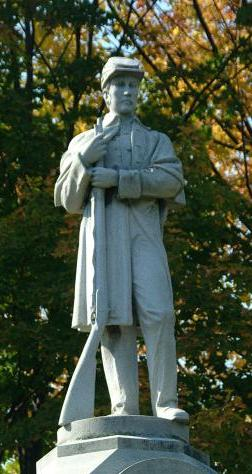
\includegraphics[scale=0.6]{scp/011.jpg}
\linebreak SCP-011
\end{center}
\end{figure}

\textbf{Special Containment Procedures:} Item SCP-011 and the area surrounding it are to be cleaned once every day. For safety purposes, cleaning should start at least 30 minutes after sundown. Cleaning should always be performed by at least two (2) personnel, who are also advised to note anything unusual about the item or the debris cleaned up. In a situation where the item cannot be cleaned for more than two (2) days, local residents must be contacted and instructed not to approach the item.

\lb Containment procedures nullified 2004\rb

\textbf{Description:} SCP-011 is a Civil War memorial statue located in Woodstock, Vermont. The statue is the image of a young male soldier holding a musket at his side, and is carved out of granite quarried within the area. Occasionally, SCP-011 has been observed lifting its musket to the sky to fire at birds which attempt to land or defecate on it. Reports detail that its movements produce soft grinding sounds but do not cause it any structural failure. Oddly, the gunfire is very similar to that of a standard firearm, despite observations that the item only loads granite bullets and granite powder into the musket (which is also unharmed by the firing). In spite of its efforts, some fecal matter does manage to strike SCP-011, and it has reportedly become distressed when it has had a large amount of feces on it, on some rare occasions even firing at humans.

\textbf{Addendum:} Those assigned to maintain SCP-011 are to see document \#011-1 for instructions.

\begin{leftbar}
\textbf{Document \#011-1: Maintenance Brief}

\lb Document archived 2004 - accessible to personnel with security clearance 2/011 or higher\rb

Additional Information: SCP-011's seeming sentience has increased since the first report of activity in 1995. As of 2004, the item's containment procedures have been dropped but it remains under constant observation. Recorded below are landmark events in its activity.

Timeline:
\begin{flushleft}
3.12.1995 - Woodstock resident reports the statue's eyes moving, first sign of activity\linebreak
9.30.1995 - Statue shoots musket for the first time\linebreak
10.9.1995 - Statue begins shooting birds from the sky\linebreak
1.25.1996 - Registration as SCP-011, containment procedures begin\linebreak
4.14.1997 - SCP-011 observed moving casually and looking around\linebreak
5.3.2000 - After caretaker \censor{XXXX} \censor{XXXXXXXX} jokingly shouts "Good shot!" to SCP-011, the item replies, "Thank you," in a reportedly very human voice, first speech from statue\linebreak
10.22.2001 - SCP-011 has conversation with caretaker \censor{XXXXXXXXX} \censor{XXXXX}
2001 - Shooting of birds stops
2.6.2002 - At the imploring of \censor{XXXXXXXXX} \censor{XXXXX}, SCP-011 steps down from its pedestal
2003-2004 - SCP-011 reaches a human level of self-awareness
11.10.2004 - Containment procedures dropped, custody of SCP-011 transferred to \censor{XXXXXXXXX} \censor{XXXXX}
5.17.2005 - \censor{XXXXXXXXX} \censor{XXXXX} reports that SCP-011 is romantically attracted to her
8.29.2006 - Most recent psych test reports an IQ of 133
\end{flushleft}
\end{leftbar}